\documentclass{ximera}

\title{A basic worksheet}
\author{Wim Obbels \and Bart Snapp}
\license{CC: 0}         % replace with an appropriate license, or set it in xmPreamble


\begin{document}
\begin{abstract}
    A simple Ximera activity.
\end{abstract}
\maketitle
\label{xim:aFirstActivity}


\section{Ideal low-pass filtering}
  Cutoff frequency $b$ (ordinary frequency, not angular)
    \begin{align*}
      \hat{h}_b(f)
      &= H_b(j2\pi f) = \operatorname{rect}(\tfrac{f}{2b})\\
      &= \begin{cases}
      1 & |\tfrac{f}{2b}| \leq \tfrac{1}{2}\\
      0 & \tfrac{1}{2} < |\tfrac{f}{2b}|
    \end{cases}\\
      &= \begin{cases}
      1 & |f| \leq b\\
      0 & b < |f|
    \end{cases}\\
      h_b(t)
      &= 2 b \sinc(2 b t) = 2 b\frac{\sin(2 \pi b t)}{2 \pi b t} = \frac{\sin(2 \pi b t)}{\pi t}
    \end{align*}

    Region of convergence for $H_b(s) = \tL{h_b}(s)$ is just the imaginary axis.\\


\subsection{Outline}
  \begin{itemize}
  \item Bandwidth
  \item Ideal filtering, rect, and sinc
  \item Approximate notions of bandwidth
  \end{itemize}
  Reading assignments: Textbook sections 6.4, 7.1-7.3


% bandwidth definition
% frequency analogue of duration
% examples: cosine, sinc, sinc^2
% derivatives and bandwidth
% approximate versions of bandwidth:
% energy/power containment
% tail decay and dependence between epsilon and bandwidth
% derivatives and approximate notions of bandwidth



\subsection{Bandwidth}
  \begin{itemize}
  \item The \emph{bandwidth} of a signal $x$ is the length of the shortest interval containing the support of the spectrum $\hat{x}$
  \item Bandwidth is the frequency-domain analogue of duration.
  \item Real signals have Hermetian spectra ($\hat{x}(-f) = \hat{x}(f)^*$), so the bandwidth of a real signal is twice the highest frequency appearing in it.
  \end{itemize}
  \vspace{2cm}


\subsection{Basic examples}
  \begin{itemize}
  \item Many signals that we have used as examples have infinite bandwidth:
    \begin{align*}
          u(t)e^{-t} &\leftrightarrow \frac{1}{1+j 2 \pi f}\\
    \exp(-\pi t^2) &\leftrightarrow \exp(-\pi f^2)
    \end{align*}
  \item Basic finite bandwidth examples:
    \begin{align*}
      \cos(2\pi a t) &\leftrightarrow \tfrac{1}{2}(\delta(f-a)+\delta(f+a))\\
      \sin(2\pi a t) &\leftrightarrow \tfrac{1}{2j}(\delta(f-a)-\delta(f+a))\\
      \sinc(at) &\leftrightarrow \tfrac{1}{a}\rect(f/a)
    \end{align*}
    What are the bandwidths of these?
    \vspace{3cm}
  \end{itemize}



\subsection{Bandwidth of a convolution}
  \begin{itemize}
  \item Convolutions in time domain correspond to pointwise product in frequency domain:
    \[
      x * y \leftrightarrow \hat{x} \odot \hat{y}
    \]
  \item The support of $\hat{x} \odot \hat{y}$ is the intersection of the supports of $\hat{x}$ and $\hat{y}$. The bandwidth is at most the minimum of the bandwidths of $x$ and $y$, but could be smaller (even zero).
  \item Putting a signal through an LTI system cannot increase its bandwidth, but it can decrease it.
  \item $x' = x * \delta'$, $\delta'(t) \leftrightarrow j2\pi f$, $x'(t) \leftrightarrow j2\pi f \hat{x}(f)$. Thus $x'$ has the same bandwidth as $x$. High frequencies components are amplified by differentiation, but they are not created from nothing.
  \end{itemize}


\subsection{Examples}



\subsection{Bandwidth of a pointwise product}
  \begin{itemize}
  \item Pointwise products in time domain correspond to convolutions in frequency domain:
    \[
      x \odot y \leftrightarrow \hat{x} * \hat{y}
    \]
  \item The support of $\hat{x} * \hat{y}$ is contained in the sum of the supports of $\hat{x}$ and $\hat{y}$. Thus the bandwidth of $x \odot y$ is the sum of the bandwidths of $x$ and $y$
  \end{itemize}
  \vspace{3cm}


\subsection{Examples}



\subsection{Ideal low-pass filtering}
  Cutoff frequency $b$, bandwidth $2b$ (ordinary frequency, not angular)
    \begin{align*}
      \hat{h}_b(f)
      &= H_b(j2\pi f) = \operatorname{rect}(\tfrac{f}{2b})\\
      &= \begin{cases}
      1 & |\tfrac{f}{2b}| \leq \tfrac{1}{2}\\
      0 & \tfrac{1}{2} < |\tfrac{f}{2b}|
    \end{cases}\\
      &= \begin{cases}
      1 & |f| \leq b\\
      0 & b < |f|
    \end{cases}\\
      h_b(t)
      &= 2 b \sinc(2 b t) = 2 b\frac{\sin(2 \pi b t)}{2 \pi b t} = \frac{\sin(2 \pi b t)}{\pi t}
    \end{align*}

    Region of convergence for $H_b(s) = \tL{h_b}(s)$ is just the imaginary axis.\\
    For any $\sigma \neq 0$, $e^{-\sigma t} h_b(t)$ is unbounded, has infinite energy, and does not have a Fourier transform.
  


\subsection{Impossibility of ideal low-pass filtering}
  Why can't we build ideal low-pass filters?
  \begin{itemize}
  \item $\sinc$ is noncausal, has infinite support, so exact implementation is impossible
  \item $\sinc$ has slowly decaying tails: As $t \to \pm \infty$, $|\sinc(t)| > \frac{c}{|t|}$ infinitely often.\\
    Any truncation faces a harsh trade-off between accuracy and duration.\\
  \item Implementing an impulse response with a long delay requires a system with lots of memory.
  \item The ideal-low pass filter is unstable:
    \[
      \int_{-\infty}^{\infty} |\sinc(t)|,dt = +\infty
    \]
    because $\sum_{n=1}^{\infty} \frac{1}{n} = +\infty$.

  \end{itemize}
 


\subsection{Delay and filtering}




\subsection{Delay and filtering}




\subsection{Delay and filtering}




\subsection{$b \to \infty$}
    \begin{align*}
      \hat{h}_b(f)
      &= \operatorname{rect}(\tfrac{f}{2b})
      = \begin{cases}
      1 & |f| \leq b\\
      0 & b < |f|
    \end{cases}\\
      h_b(t)
      &= 2 b \sinc(2 b t) = \frac{\sin(2 \pi b t)}{\pi t}
    \end{align*}
What happens to $\hat{h}_b$ and $h_b$ as $b \to \infty$?
\begin{align*}
  \hat{h}_b(f) &\to 1\\
  \tFi{1}(t) &=\delta(t)\\
\end{align*}
The frequency response approach one, the response of an identity/all-pass system.\\
Does the impulse response approach a Dirac delta?


\subsection{Plots}
  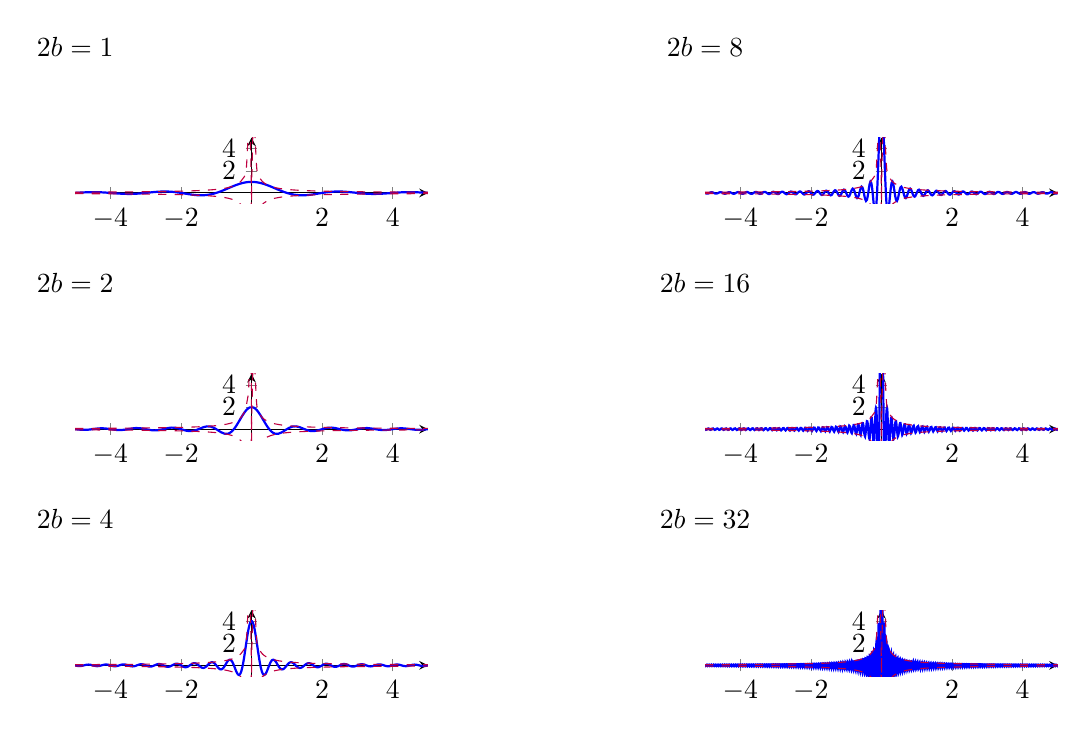
\begin{tikzpicture}
    \begin{scope}[shift={(0,0)}]
      \node at (0,2) {$2b=1$};
      \begin{axis}[
        xmin = -5, xmax = 5,
        ymin = -1, ymax = 5,
        xtick distance = 2,
        ytick distance = 2,
        axis x line = middle,
        axis y line = middle,
        width = 0.5\textwidth,
        height = 0.2\textwidth,
        ]           
          
          \addplot[
          smooth,
          thick,
          blue,
          samples=100,
          ]{sin(180*x)/pi/x}; %sin takes degrees
          
          \addplot[
          smooth,
          dashed,
          purple,
          samples=100,
          ]{1/pi/x};
                    
          \addplot[
          smooth,
          dashed,
          purple,
          samples=100,
          ]{-1/pi/x};
        \end{axis}
      \end{scope}
      \begin{scope}[shift={(0,-3)}]
              \node at (0,2) {$2b=2$};
      \begin{axis}[
          xmin = -5, xmax = 5,
          ymin = -1, ymax = 5,
          xtick distance = 2,
          ytick distance = 2,
          axis x line = middle,
          axis y line = middle,
          width = 0.5\textwidth,
          height = 0.2\textwidth,
          ]           
          
          \addplot[
          smooth,
          thick,
          blue,
          samples=100,
          ]{sin(360*x)/pi/x}; %sin takes degrees
          
          \addplot[
          smooth,
          dashed,
          purple,
          samples=100,
          ]{1/pi/x};
                    
          \addplot[
          smooth,
          dashed,
          purple,
          samples=200,
          ]{-1/pi/x};
        \end{axis}
      \end{scope}
      \begin{scope}[shift={(0,-6)}]
        \node at (0,2) {$2b=4$};
        \begin{axis}[
          xmin = -5, xmax = 5,
          ymin = -1, ymax = 5,
          xtick distance = 2,
          ytick distance = 2,
          axis x line = middle,
          axis y line = middle,
          width = 0.5\textwidth,
          height = 0.2\textwidth,
          ]           
          
          \addplot[
          smooth,
          thick,
          blue,
          samples=400,
          ]{sin(720*x)/pi/x}; %sin takes degrees
          
          \addplot[
          smooth,
          dashed,
          purple,
          samples=100,
          ]{1/pi/x};
                    
          \addplot[
          smooth,
          dashed,
          purple,
          samples=100,
          ]{-1/pi/x};
        \end{axis}
      \end{scope}
    \begin{scope}[shift={(8,0)}]
      \node at (0,2) {$2b=8$};
      \begin{axis}[
        xmin = -5, xmax = 5,
        ymin = -1, ymax = 5,
        xtick distance = 2,
        ytick distance = 2,
        axis x line = middle,
        axis y line = middle,
        width = 0.5\textwidth,
        height = 0.2\textwidth,
        ]           
          
          \addplot[
          smooth,
          thick,
          blue,
          samples=400,
          ]{sin(1440*x)/pi/x}; %sin takes degrees
          
          \addplot[
          smooth,
          dashed,
          purple,
          samples=100,
          ]{1/pi/x};
                    
          \addplot[
          smooth,
          dashed,
          purple,
          samples=100,
          ]{-1/pi/x};
        \end{axis}
      \end{scope}
      \begin{scope}[shift={(8,-3)}]
              \node at (0,2) {$2b=16$};
      \begin{axis}[
          xmin = -5, xmax = 5,
          ymin = -1, ymax = 5,
          xtick distance = 2,
          ytick distance = 2,
          axis x line = middle,
          axis y line = middle,
          width = 0.5\textwidth,
          height = 0.2\textwidth,
          ]           
          
          \addplot[
          smooth,
          thick,
          blue,
          samples=400,
          ]{sin(2880*x)/pi/x}; %sin takes degrees
          
          \addplot[
          smooth,
          dashed,
          purple,
          samples=100,
          ]{1/pi/x};
                    
          \addplot[
          smooth,
          dashed,
          purple,
          samples=100,
          ]{-1/pi/x};
        \end{axis}
      \end{scope}
      \begin{scope}[shift={(8,-6)}]
        \node at (0,2) {$2b=32$};
        \begin{axis}[
          xmin = -5, xmax = 5,
          ymin = -1, ymax = 5,
          xtick distance = 2,
          ytick distance = 2,
          axis x line = middle,
          axis y line = middle,
          width = 0.5\textwidth,
          height = 0.2\textwidth,
          ]           
          
          \addplot[
          smooth,
          thick,
          blue,
          samples=800,
          ]{sin(5760*x)/pi/x}; %sin takes degrees
          
          \addplot[
          smooth,
          dashed,
          purple,
          samples=100,
          ]{1/pi/x};
                    
          \addplot[
          smooth,
          dashed,
          purple,
          samples=100,
          ]{-1/pi/x};
        \end{axis}
      \end{scope}
    \end{tikzpicture}


\subsection{Weak convergence to Dirac delta}
  \begin{itemize}
  \item As $b \to \infty$, the oscillation becomes faster within a fixed envelope
  \item $\lim_{b \to \infty} h_a(0) =+\infty$ and for $t\neq 0$, $\lim_{b \to \infty} h_b(0)$ does not exist.
  \item For $t \neq 0$, the envelope $\pm \frac{1}{\pi t}$ is continuous, as thus approximately constant at small scales. Consecutive positive and negative oscillations almost exactly cancel.
  \item Around $t = 0$, there is a positive bump that does is not fully canceled by the adjacent negative bumps.
  \item For any finite energy signal $x$,
    \[
      \lim_{b \to \infty} \langle h_b, x\rangle = \lim_{b \to \infty} \int_{-\infty}^{\infty} \frac{\sin(2 \pi b t)}{\pi t} x(t)\,dt \to x(0) = \langle\delta,x\rangle
    \]
  \item Be careful with the statement $\delta(t) = 0$ for $t \neq 0$.
  \end{itemize}


\subsection{Weak convergence to Dirac delta}

      The integral of $h_b$ converges to the integral of $\delta$: 
    \begin{align*}
      &\lim_{b \to \infty}  \int_{-\infty}^t h_b(\tau)\,d\tau\\
      &= \lim_{b \to \infty}  \int_{-\infty}^t \frac{\sin(2 \pi b t)}{\pi t}
\,d\tau\\
      &= \begin{cases}
        0 & t < 0\\
        \tfrac{1}{2} & t=0\\
        1 & t >0
      \end{cases}
    \end{align*}
  
\includegraphics[width=\textwidth]{618px-Sine_integral.svg.png}\\
Image created by wikipedia user Krishnavedala for the article ``Sine integral''.



\subsection{Review: Sinc and ideal filtering}
  \begin{itemize}
  \item $\sinc(t) = \frac{\sin(\pi t)}{\pi t}$
  \item
    \[
      \tF{\sinc}(f) = \rect(f) = \begin{cases}
        1 & -\tfrac{1}{2} \leq f \leq \tfrac{1}{2}\\
        0 & \text{otherwise}
      \end{cases}
    \]
    \item Ideal low-pass filter with cut-off frequency $b > 0$:
    \[
      2b \sinc(2bt) \leftrightarrow \rect(\tfrac{f}{2b})
    \]
  \item The sinc pulse is non-causal and even, decays slowly at rate $\tfrac{1}{t}$ due to the discontinuity in rectangle pulse
  \item As $b \to \infty$, $\rect(\tfrac{f}{2b}) \to 1$ (pointwise and in other senses)

    $2b \sinc(2bt) \to \delta(t)$ (but does not converge pointwise)
  \end{itemize}


\subsection{Ideal high pass filtering}
  To find the ideal high-pass filter with cutoff frequency $b$, take the difference between all-pass and low-pass filters:
    \begin{align*}
      \hat{h}(f) &= 1 - \rect(\tfrac{f}{2 b})\\
      h(t) &= \delta(t) - 2 b \sinc(2 b t)
    \end{align*}


  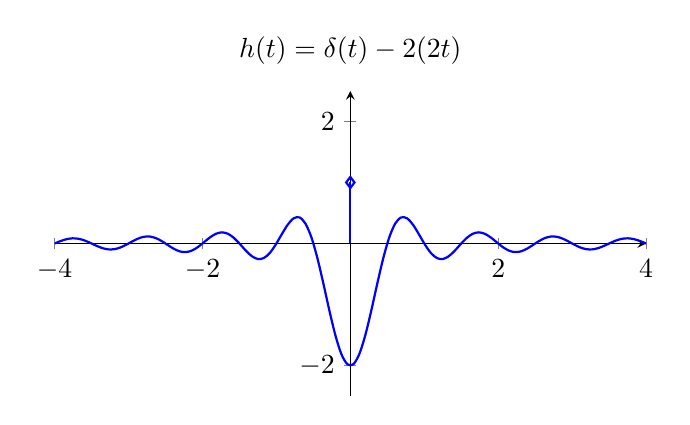
\begin{tikzpicture}
        \begin{axis}[
          title = {$h(t) = \delta(t)-2 \sinc(2 t)$},
        xmin = -4, xmax = 4,
        ymin = -2.5, ymax = 2.5,
        xtick distance = 2,
        ytick distance = 2,
        axis x line = middle,
        axis y line = middle,
        width = 0.75\textwidth,
        height = 0.45\textwidth,
        ]           
          

          \addplot[
          smooth,
          thick,
          blue,
          domain = -4:4,
          samples=100,
          ]{-sin(360*x)/pi/x};

          \addplot+ [ycomb,mark=diamond,blue,thick] coordinates {(0,1)};
        \end{axis}

    \end{tikzpicture}



\subsection{Approximate notion of bandwidth}
  \begin{itemize}
  \item Many fundamental examples of signals have infinite bandwidth, but their spectra decay rapidly as $f \to \infty$ 
  \item The basic definition of bandwidth is not robust to small changes in the signal.
  \item For these two reasons, modified versions of the definition of bandwidth are very useful in practice.
  \item \emph{$1-\epsilon$-energy/power-containment bandwidth} and \emph{dispersion in frequency} are two approximate notions of bandwidth
  \end{itemize}
  \vspace{3cm}


\subsection{Energy/power containment bandwidth}



\subsection{Dispersion in frequency}
We can measure the bandwidth of a signal centered at frequency zero using the energy spectral density:
  \[
    \frac{1}{\|\hat{x}\|^2} \int_{-\infty}^{\infty} f^2 |\hat{x}(f)|^2 df
  \]

$\frac{|\hat{x}(f)|^2}{\|\hat{x}\|^2}$ is a probability density, so this is the second moment of a random variable. 


  


\subsection{Approximate bandwidth of low-pass impulse response}




\subsection{Derivatives and approximate notions of bandwidth}
  \begin{itemize}
  \item
    Differentiation \emph{can} increase approximate bandwidth.\\
    It increases the relative weight of higher frequencies.
  \item High frequencies that were contributed only $\epsilon$-fraction of the energy in the original signal will contributed a larger fraction in the derivative. Thus, a higher cutoff will be required to cover $1-\epsilon$ fraction of the energy in the derivative.
  \item The decay rate of the spectrum determines how much larger the bandwidth of the derivative is.
  \end{itemize}




\end{document}
